
%% Commands for TeXCount
%TC:macro \cite [option:text,text]
%TC:macro \citep [option:text,text]
%TC:macro \citet [option:text,text]
%TC:envir table 0 1
%TC:envir table* 0 1
%TC:envir tabular [ignore] word
%TC:envir displaymath 0 word
%TC:envir math 0 word
%TC:envir comment 0 0
%% EAdejumo: converted from acmart (sigconf) to IEEEtran conference format for SANER submission.
%% All ACM-specific rights-management/template boilerplate below has been removed since it has
%% no IEEEtran equivalent and would not compile; package loads that acmart provided implicitly
%% (xcolor, graphicx, amsmath/amssymb, cite) are now made explicit.
\documentclass[10pt,conference]{IEEEtran}
\usepackage{xcolor}
\usepackage{graphicx}
\usepackage{amsmath}
\usepackage{amssymb}
\usepackage{hyperref} 
\usepackage{cite}
\newcommand{\BJohnson}[1]{\textcolor{purple}{{\bfseries [[#1]]}}}
\newcommand{\EAdejumo}[1]{\textcolor{red}{{\bfseries [[#1]]}}}
\newcommand{\MGuizani}[1]{\textcolor{blue}{{\bfseries [[#1]]}}}
\usepackage{enumitem}
\usepackage{booktabs}
\usepackage[utf8]{inputenc}
\usepackage{textcomp}
\definecolor{heatmaplight}{HTML}{DBEAFE}
\definecolor{heatmapdark}{HTML}{1F4E79}
\usepackage{multirow}
\usepackage{tcolorbox}

\begin{document}


\title{Empirical Characterization of Health Documentation Governance in Open Source Projects}



\maketitle

\begin{abstract}
Open Source Software (OSS) health documentation comprises of files that govern how users or contributors join, interact with, and sustain an open source project; these artifacts are essential to project sustainability, yet their governance is not clearly understood.
We present a decade-long empirical characterization of documentation governance across 100 open source repositories, examining 37,447 health documentation commits through three lenses: rhythm, intention, and ownership.
We identify three distinct documentation rhythm archetypes (Consistent (37\%), Occasional (50\%), and Sparse (13\%)
Documenters), demonstrating that documentation maintenance
follows structured recurring patterns rather than random activity, and we further show that this rhythm structure is durable: Consistent and Sparse Documenters persist as the same archetype from one year to the next 76\% and 62\% of the time respectively, while Occasional functions as a transitional state repositories pass through rather than settle into.
We found ownership to be concentrated in a minority of contributors, with the median repository relying on only 6.3\% of its contributor base for health documentation.
Tracking these dimensions across the full decade studied, however, shows documentation governance is not static: the breadth of contributor participation and the deliberateness of documentation activity have each declined significantly as projects mature, even as rhythm archetypes remain stable, and self-reinforcing, once established.

Critically, we show this ownership structure is not merely descriptive but predictive, and that its two facets pull in different directions: documentation bus factor independently predicts documentation staleness beyond project size and documentation volume, while the breadth of documentation participation independently predicts \textit{lower} retention of individual documentation newcomers, a reach-versus-persistence tradeoff rather than a uniform benefit.
We discuss implications for repository health tooling, contributor onboarding, and the operationalization of documentation governance as a measurable, outcome-relevant, and evolving dimension of OSS sustainability.
\end{abstract}

% \begin{IEEEkeywords}
% open source software, documentation governance, repository mining, bus factor, contributor retention, mining software repositories
% \end{IEEEkeywords}

\section{Introduction}
Open source software (OSS) has become a critical component of global software supply-chain infrastructure, contributing billions of dollars in value across the globe with more than 90\% of commercial software containing one or more OSS project \cite{hoffmann2024value,nagle2019open}.
The centrality of OSS is further emphasized by widespread support provided by  large companies and organizations including Google, Nvidia, Linux Foundation, Apache \cite{linux_foundation,google_opensource,apache_foundation} to help sustain OSS ecosystems. Despite the growing importance and value of OSS, it continues to face significant challenges that threaten its long-term sustainability. 
For an OSS ecosystem to stand the test of time, projects must remain stable and robust in the face of changing contributors, processes, codebases, and evolving needs \cite{bouktif2014predicting,destefanis2025introducing}. 
Therefore, ensuring that knowledge and practices persist over time is  essential to maintaining and sustaining project quality.


% Among the relevant considerations, governance and coordination of open infrastructure such as OSS ecosystems stand out as critical factors based on a growing body of research \cite{shaikh2017governing,di2013governance} that has investigated how  communities coordinate and govern their development over time.
Prior work has examined several dimensions of OSS governance, including how code contributions are committed to repositories, how pull requests and issues are managed, and how newcomers are on-boarded into a project\cite{aufiero2026coordination,arya2019analysis,steinmacher2014attracting,alami2021pull}. 
However, while documentation serves as a essential medium through which coordination and governance norms are communicated within OSS ecosystems, no study has yet examined how health documentation~\cite{github_community_health}, a crucial coordination and governance artifact in OSS projects, is itself governed and coordinated across projects.
This is particularly concerning given that documentation such as \textsc{ReadMe.md} and \textsc{Contributing.md} serve as critical entry points for newcomers \cite{gaughan2025introduction, adejumo2026bridging}, while other artifacts such as \textsc{Security.md}, \textsc{Code\_of\_Conduct.md}, and \textsc{Governance.md} \cite{github_community_health} play a vital role in facilitating knowledge sharing around processes, governance, and policies ultimately reducing coordination friction across OSS ecosystems. 

While the importance of OSS documentation cannot be denied ~\cite{coelho2017modern}, it has largely been studied from a static perspective focusing primarily on availability and quality dimensions such as whether it adequately addresses developers' needs, its correctness, currency, and freedom from misleading information \cite{aversano2017evaluating}. This static lens creates a critical gap in our  understanding of how documentation maintenance, coordination, and governance unfold as measurable, dynamic processes over time. 
To fill this gap, we conducted an empirical study to investigate how OSS projects maintain crucial documentation \cite{github_community_health} over time, examining maintenance rhythm, the intention behind maintenance, and the contributors who drive it. 
These three dimensions, established in the OSS governance literature ~\cite{shaikh2017governing}, characterize governance in terms of coordination processes, contributor activity, and authoritative structures, all of which are shaped by community norms. We operationalize these components as rhythm, ownership, and intention, respectively. Rhythm captures how documentation coordination processes recur over time, ownership reflects who holds authority over documentation, and intention distinguishes whether documentation changes are deliberate or incidental. Each dimension is also grounded in prior empirical work. Rhythm ~\cite{adejumo2026commits,destefanis2025introducing}. Ownership ~\cite{cosentino2015assessing,jabrayilzade2022bus}, and intention ~\cite{zeng2025first}, we treat them as the measurable components of a single governance duality already established in theory, applied here to health documentation. 
% \EAdejumo{RQ3 reworded to fold in outcome validation; a fourth contribution added summarizing the predictive-validity results integrated into RQ3.}

Our investigation was guided by the following research questions:
\begin{description}
    \item \textbf{RQ1} What documentation rhythm patterns characterize OSS repositories, and how are these patterns distributed across projects? 
    \item \textbf{RQ2} To what extent do OSS contributors exhibit intentional documentation behavior?
    \item \textbf{RQ3} How is documentation ownership distributed across contributors, and does this ownership structure predict downstream project outcomes?
    \item \textbf{RQ4} Are documentation rhythm, intention, and ownership stable properties of a project, or do they shift as it matures over a decade of observation?
\end{description}

Our findings surface four central results. We identify three distinct documentation rhythm archetypes, Consistent, Occasional, and Sparse, showing that when projects document at all, they typically do so in irregular bursts rather than as a sustained, ongoing practice \textbf{(RQ1)}. Using a novel commit-level intention taxonomy (DocOnly, DocDominant, DocNonDominant), we show documentation activity is rare but deliberate when it occurs \textbf{(RQ2)}. Applying bus factor analysis to health documentation for the first time, we find ownership structurally fragile, and show this structure is not only descriptive: documentation bus factor independently predicts documentation staleness, while documentation participation breadth independently predicts \textit{lower} retention of individual documentation newcomers, both beyond project size and activity volume, revealing a reach-versus-persistence tradeoff rather than a single dominant governance lever \textbf{(RQ3)}. Finally, tracking each dimension annually across the decade reveals that rhythm archetypes are durable and self-reinforcing once established, Consistent and Sparse Documenters persist as the same archetype year over year 76\% and 62\% of the time respectively, while the deliberateness and breadth of documentation engagement have each declined significantly over the same window \textbf{(RQ4)}.






% Our research contributes the following: \textbf{(i) } the first large-scale empirical characterization of project health documentation governance across 100 mature OSS repositories through three independently measured lenses; \textbf{(ii)} a commit-level documentation intention taxonomy (DocOnly, DocDominant, DocNonDominant) that
% distinguishes deliberate from incidental documentation behavior; \textbf{(iii)} the first application of bus factor analysis specifically to project health documentation commits, revealing structural fragility
% invisible to code-centric health frameworks; \textbf{(iv)} outcome-validated evidence that documentation ownership structure, specifically contributor participation breadth and documentation bus factor, independently predicts documentation staleness and contributor retention beyond project size and activity volume, giving these governance metrics demonstrated predictive value rather than descriptive value alone.

% \EAdejumo { we found that ................}



% \EAdejumo{Being you seem to be using a more non-traditional format for the paper, I would recommend having a paragraph here at the end of the intro that summarizes the paper organization. I've added labels to the sections that are here so far and added some starter text to give an idea of what I mean.}


% The remainder of this paper is organized as follows. In Section~\ref{sec:related_work}, we outline existing research related to our efforts. Section \ref{sec:dataset_const} describes dataset construction, Section \ref{sec:RQ1}---\ref{sec:RQ3} presents methodology and findings for RQ1, RQ2, and RQ3 respectively. Section \ref{sec:Discussion} discusses implications. Section \ref{sec:Threats_to_Validity} addresses the threats to validity and Section \ref{sec:conclusion} concludes.




\section{Related Work}~\label{sec:related_work}

% \noindent \textbf{ {OSS Sustainability and Project Health: }}
% The sustainability of OSS has been a critical research concern for more than a decade \cite{gamalielsson2014sustainability,alami2024free}, with all stakeholders maintainers, contributors, and adopters  playing significant roles in ensuring its long-term viability. However, sustaining an OSS project is far from straightforward, as the ecosystem faces challenges from multiple fronts.
% Newcomers are vital to OSS sustainability, as they typically begin as users and bug reporters before gradually transitioning into contributors and eventually core team members \cite{aberdour2007achieving}. Despite their importance, newcomers frequently encounter barriers that are social, technical, or both hindering their ability to integrate and contribute effectively \cite{steinmacher2015social,adejumo2024towards,adejumo2025explaining}. On the other side of the ecosystem, maintainers face their own set of challenges, including burnout, task coordination, and governance overhead, all of which are compounded by the voluntary nature of OSS contribution \cite{linaaker2024sustaining,tan2023enough}. Project health metrics, on the other hand, provide measurable insights into the overall state of an OSS project, serving as valuable signals for adopters, downstream consumers, and supply chain utilization decisions. Key indicators such as commit activity, issue resolution rates, pull request merge rates, bus factor and contributor churn and retention have been widely studied as proxies for project vitality and long-term sustainability \cite{goggins2021open,destefanis2025introducing}.

\noindent \textbf{ {Documentation in software engineering and OSS:}}
The importance of good software documentation cannot be overstated, it is fundamental to the use, maintenance, adoption, and evolution of any software system \cite{aghajani2020software}. This holds equally true for OSS projects, where documentation quality has been extensively studied and tools and methods have been developed to assess it \cite{aversano2017evaluating,carvalho2013open}.
Among the most studied artifacts is the \texttt{README.md} file, which typically serves as the primary entry point for users visiting a repository \cite{adejumo2026bridging}. Given its visibility and influence, numerous methods and techniques have been proposed to improve its creation, quality, and maintenance \cite{liu2022readme,gaughan2025introduction}. Beyond the \texttt{README.md}, other project health documentation artifacts play equally important roles across different dimensions of OSS project health. Files such as \texttt{Contributing.md}, \texttt{Security.md}, \texttt{Code \_of \_Conduct.md}, and \texttt{Governance.md} govern onboarding, security practices, community behavior, and project governance, respectively, and have attracted growing research interest, with methods and techniques proposed to improve and maintain them \cite{kobayakawa2017github,adejumo2024towards,tufano2024unveiling}.
These prior contributions are largely motivated by evidence that the quality, accessibility, freshness, and readability of such documentation are key factors in successful contributor onboarding, security posture, governance effectiveness, and the overall sustainability of OSS ecosystems \cite{steinmacher2014attracting, adejumo2025explaining,steinmacher2015social,adejumo2026bridging,choetkiertikul2026security}. 

\noindent \textbf{ { Project Health, Coordination and Governance in OSS:}}
Project health metrics provide measurable insights into the overall state of an OSS project, serving as valuable signals for adopters, downstream consumers, and supply chain utilization decisions. Key indicators such as commit activity, issue resolution rates, pull request merge rates, bus factor and contributor churn and retention have been widely studied as proxies for project vitality and long-term sustainability \cite{goggins2021open,destefanis2025introducing}. Unlike traditional software development, where coordination and governance are typically enforced through formal organizational structures, OSS ecosystems operate under fundamentally different dynamics. As OSS adoption has grown, understanding how coordination and governance function within these ecosystems has become increasingly critical particularly how the relationships between contributors influence project sustainability, a dimension that has been extensively studied through a socio-technical lens \cite{bird2011sociotechnical,aufiero2026coordination}.
Shaikh et al. \cite{shaikh2017governing} investigated the duality of coordination and governance in OSS, finding that both operate in parallel and are mutually reinforcing. Their work further characterizes governance as encompassing shared rules, norms, and instructions, alongside activities that operationalize the authoritative structure of an ecosystem  with common coordination patterns observable directly from version control system activity.
Beyond contributor interactions, documentation artifacts serve as a complementary mechanism for facilitating coordination and governance in OSS projects \cite{github_community_health}, codifying the norms and expectations that guide how contributors engage with and sustain the ecosystem over time.
These efforts, however, characterize governance at a single point in time; whether the resulting patterns are stable properties of a project or drift as it matures over a multi-year horizon remains largely unexamined, a gap prior temporal work on OSS commit rhythms \cite{destefanis2025introducing,adejumo2026commits} has begun to address for code but not documentation. We address this directly by tracking documentation rhythm, intention, and ownership annually across a full decade (RQ4).

% \subsection{Temporal maintenance patterns and software evolution}

% Understanding temporal activity patterns  including stability patterns has been a recurring theme in software engineering research. Prior studies have proposed methods leveraging version control data to characterize and predict OSS stability \cite{bouktif2014predicting,raemaekers2012measuring}. More recently, research using pull request merge rates and issue resolution times rhythms serve as insightful signals of OSS project health \cite{destefanis2025introducing,adejumo2026commits}, drawing on control theory principles where stable, consistent processes in manufacturing tend to yield more predictable and higher-quality outcomes.

% Building on this body of work, this study extends the temporal lens beyond code contributions to examine the maintenance rhythms, commit intentions, and ownership patterns of community health documentation across 100 mature, highly-ranked OSS repositories.


\section{Dataset Construction}\label{sec:dataset_const}
% To reveal how documentation coordination and governance unfold in OSS ecosystems, we conducted a large-scale empirical study examining repository-level maintenance activity over time through three analytical lenses: \textit{rhythm}, or the temporal patterns of documentation updates, \textit{intention}, or the purpose and motivation behind each change, and \textit{ownership}, or the contributors responsible for driving and sustaining documentation maintenance.

\textbf {Repository Selection:}
\label{Repository_Selection}
For this study, we selected the top 100 repositories based on the following criteria, which we deemed most relevant to our research questions:

\noindent \textbf{Community Interest (Stars $>$ 10,000)}: We prioritized 
repositories with high star counts as a proxy for sustained community 
interest and visibility \cite{borges2018s}, reflecting significant 
engagement and adoption across the developer community over time.

\noindent \textbf{Maturity ($\ge$ 10 Years)}: We selected repositories that 
are at least a decade old, as they provide sufficient historical depth 
to observe stable maintenance patterns, long-term evolutionary trends, 
and well-established governance practices.

\noindent \textbf{Active Adoption (Forks $>$ 9,000)}: We focused on 
repositories with substantial fork counts, as forking activity reflects 
real-world usage and downstream adoption within the broader developer 
community \cite{jiang2017and}.
    
\noindent \textbf{Software Development Focus}: We excluded repositories 
primarily serving educational purposes including those containing 
books, programming tutorials, videos, and instructional materials 
to ensure our dataset reflects genuine software development dynamics 
rather than curated learning content.
    
\noindent \textbf{Active Status}: We excluded archived repositories during 
manual filtering to ensure our dataset consists of currently active 
projects that continue to evolve, attract contributions, and undergo 
meaningful maintenance activity.
    
\noindent \textbf{Activity Window (2016-2026)} :
We use the most recent decade as the observation window to estimate documentation activity patterns in a comparable mature phase across repositories, and to support a within-study evolution analysis (RQ4, Section~\ref{sec:RQ4}) that a shorter window cannot support. Each repository in our sample was verified to have commit history predating this window by a comfortable margin, ensuring the full decade falls within each project's mature, post-bootstrapping lifecycle rather than overlapping its founding period.

\textbf{Project Health Documentation:}
\label{sec:Health_docs}
We define \textbf{project health documentation} as repository-residing documentation artifacts that directly support project governance, contributor coordination, and community continuity. 
In contrast to other technical documentation (e.g., API references, tutorials, or feature-specific manuals), health documentation captures the operational and social infrastructure of a project: how contributors enter, participate in, and align with project norms. 
These artifacts, labeled as community health documents by GitHub \cite{github_community_health}, support stable coordination processes that shape on-boarding, participation expectations, reporting pathways, and maintenance practices, making them especially relevant to the study of documentation governance and OSS sustainability.
The specific documentation artifacts included in our analysis are shown in Table~\ref{tab:documentation_artifacts}.
\vspace{-10pt}
\begin{table}[h]
\centering
\caption{Health Documentation Artifacts}
\label{tab:documentation_artifacts}
\renewcommand{\arraystretch}{1.3}
\begin{tabular}{p{3.5cm}p{4.5cm}}
\hline
\textbf{Artifact} & \textbf{Description} \\
\hline
\texttt{README} & Primary entry point and project overview \\
\texttt{CONTRIBUTING} & Guidelines for contributing \\
\texttt{CONTRIBUTORS} & List of project contributors \\
\texttt{COMMIT\_CONVENTIONS} & Commit message standards \\
\texttt{BUILDING} & Build instructions \\
\texttt{PULL\_REQUEST\_TEMPLATE} & Template for pull requests \\
\texttt{ISSUE\_TEMPLATE} & Template for issue reporting \\
\texttt{CHANGELOG} & Log of changes across versions \\
\texttt{HISTORY} & Historical record of changes \\
\texttt{RELEASE(S)} & Release notes and announcements \\
\texttt{CODE\_OF\_CONDUCT} & Community behavior standards \\
\texttt{GOVERNANCE} & Governance structure and policies \\
\texttt{SUPPORT} & Guidance for obtaining support \\
\texttt{MAINTAINERS} & List of active maintainers \\
\texttt{SECURITY} & Vulnerability reporting policy \\
\texttt{LICENSE} & Project license terms \\
\texttt{NOTICE} & Legal notices and attributions \\
\texttt{COPYING} & Copying and distribution terms \\
\texttt{AUTHORS} & Official list of project authors \\
\texttt{CREDITS} & Contributor acknowledgments \\
\texttt{THANKS} & Recognition of supporters \\
\texttt{ROADMAP} & Planned development directions \\
\texttt{VISION} & Long-term goals and philosophy \\
\hline
\end{tabular}
\end{table}


\textbf{Data Extraction:}
We locally cloned all 100 repositories selected based on our inclusion criteria (Section~\ref{Repository_Selection}) and extracted documentation-related commits from their version histories using native Git commands. For each repository, we collected commit-level metadata, including the commit hash, author identity, timestamp, commit message, the specific health documentation files modified in each commit, and each commit's automated-vs-human authorship status to support bot filtering and identity normalization (Section~\ref{sec:RQ3}). These data enabled our analysis of documentation maintenance rhythm, intention, and ownership. Automated actors are excluded from all ownership and structural-fragility calculations throughout; where rhythm metrics are affected by automated commit activity, we report a dedicated robustness check (Section~\ref{sec:RQ1}, Artifact-Type and Bot Robustness).


\section{METHODOLOGY}
\subsection{ Documentation Rhythm Patterns, Characteristics, \& Distribution (RQ1) }\label{sec:RQ1}

% Documentation maintenance rhythm is a temporal fingerprint that
% can reveal a project's documentation governance culture; prior work shows that temporal engagement patterns (e.g., consistent vs. seasonal activity) reflect underlying community dynamics, stability, and coordination practices in OSS projects \cite{ouf2026empirical} and temporal commit patterns can serve as insightful signals of OSS project health and coordination dynamics~\cite{destefanis2025introducing, adejumo2026commits, shaikh2017governing}. Building on this, we view documentation maintenance rhythms as a similar temporal signal that is a
% crucial step towards improving documentation governance at scale.

% \EAdejumo{Do we have a cite for this? the first part in particular...I watered it down a bit but reviewers might still wonder what the importance of documentation rhythms are...even if the cite is about other OSS rhythms as indicators or community culture could help.}

% \MGuizani{Mariam: I suggest combining problem addressed and gap as they tackle the same aspect. We can call it "motivation and research gap". Right now research gap and problem addressed is a at lower title level than Approach which might raise some readability/ strcuture questions from reviewers}
\textbf{Motivation and Problem Addressed:}
Existing OSS health metrics~\cite{chaoss} treat documentation as a binary or volumetric construct (e.g., either a project has documentation or it does not) where more is generally assumed to be better. 
Particularly, measures of documentation tend to focus on file count, coverage measurement, or quality assessment at a single point in time. 
What none of these approaches capture is the temporal dimension, which is whether documentation activity is sustained, regular, and deliberate over time, or whether it happens in isolated bursts separated by long periods of neglect. This distinction is consequential, prior work has established that temporal commit rhythms  correlate with project health
indicators such as contributor concentration and sustainability
risk ~\cite{destefanis2025introducing, adejumo2026commits}. Documentation maintenance rhythm refers to the temporal regularity with which a project sustains documentation activity over time.
We further evaluate documentation maintenance rhythm at a monthly granularity, which prior work identified as a feasible and meaningful unit of analysis for understanding maintenance patterns within OSS ecosystems~\cite{adejumo2026commits}. 
Building on this, we operationalize documentation maintenance rhythm across 121 months spanning a decade-long observation period.
Additionally, we evaluate an active window rate, defined as the proportion of months within the observation period in which at least one documentation maintenance commit was recorded, capturing the breadth of sustained documentation activity across the evaluation window.


% No prior empirical study has characterized documentation rhythm as a measurable construct across a large sample of OSS repositories. The CHAOSS project \cite{chaoss}, the most comprehensive OSS health framework available, defines dozens of metrics for code activity, contributor engagement, and community health but has no metric for documentation processes over time. 
% Previous studies that examine documentation in OSS have focused on documentation quality, coverage gaps, or onboarding effectiveness
% \cite{steinmacher2014attracting,adejumo2024towards,carvalho2014dmoss}, and none considered the documenting processes in OSS. Without understanding documentation rhythm, it becomes difficult to distinguish between steady documentation and bursty documentation practices. Both may appear identical in volume and even score similarly on readability or coverage metrics, yet reflect fundamentally different governance cultures and sustainability trajectories.

 
% Unlike a single snapshot of documentation-related commit volume, rhythm captures how consistently documentation is maintained as an ongoing process and practice. 
% To measure and operationalize this, we employed Shannon Entropy, a rhythm-based metric that has been applied in software engineering studies to characterize variability and regularity in development activity \cite{hassan2009predicting,eyolfson2011time,destefanis2025introducing}. 

{\textbf{Normalized Shannon Entropy:}
Let $x_1, x_2, \dots, x_M$ denote the number of health documentation related commits observed in each monthly window over the analysis period, where 
$M = 121$ is the total number of months in the observation window.

% We define 
% the proportion of total documentation activity occurring in month $i$ as
% \[
%   p_i = \frac{x_i}{\sum_{j=1}^{M} x_j}.
% \]
The Shannon entropy is computed as
\[
  H = - \sum_{i=1}^{M} p_i \log_2 p_i,
\]
where terms with $p_i = 0$ are treated as contributing $0$ (consistent with 
the standard convention $\lim_{p \to 0} p \log_2 p = 0$). We normalize entropy using it's theoretical maximum to account for 
the length of the observation window.
\[
  H_{\mathrm{norm}} = \frac{H}{\log_2 M}.
\]
This yields $H_{\mathrm{norm}} \in [0, 1]$, where values approaching $1$ 
indicate documentation activity distributed evenly across months, and values 
approaching $0$ indicate activity concentrated in few months.

% \subsubsection{\textbf{ Coefficient of Variation (CV)} }

% Let $x_1, x_2, \dots, x_M$ denote the number of health documentation commits observed in each monthly window over the analysis period, where $M$ is the total number of months. The mean monthly activity is

% \[
% \mu = \frac{1}{M}\sum_{i=1}^{M} x_i
% \]

% and the sample standard deviation is

% \[
% \sigma = \sqrt{\frac{1}{M-1}\sum_{i=1}^{M}(x_i - \mu)^2 }.
% \]

% The coefficient of variation is then defined as

% \[
% CV = \frac{\sigma}{\mu}.
% \]

% Lower values indicate more stable documentation activity over time, while higher values indicate greater volatility or burstiness.

\textbf{Active Window Rate (AWR):}
Let $x_i$ denote the number of health-file documentation commits in month 
$i$, for $i = 1, \dots, M$, using the same observation window as defined 
above ($M = 121$ months). We define an indicator function for whether a
month contains any documentation activity:
\[
  \mathbf{1}(x_i > 0) =
  \begin{cases}
    1, & \text{if month } i \text{ contains at least one} \\
       & \text{health-file documentation commit,} \\
    0, & \text{otherwise.}
  \end{cases}
\]
The Active Window Rate is then defined as
\[
  \mathit{AWR} = \frac{1}{M} \sum_{i=1}^{M} \mathbf{1}(x_i > 0).
\]
$\mathit{AWR} \in [0, 1]$, where $\mathit{AWR} = 1$ indicates documentation 
activity in every observed month and $\mathit{AWR} \approx 0$ indicates 
near-complete absence of documentation activity across the window. 
 $\mathit{AWR}$ measures the continuity of documentation presence across the full window capturing whether extended documentation gaps exist regardless of how active the project is when it does document.
\textbf{Maintenance Patterns across OSS Ecosystem:} To reveal maintenance rhythms across the OSS ecosystems we utilize K-means Clustering \cite{mcqueen1967some} with $n\_init = 10$ random initializations which retains the solution within the lowest inertia to mitigate sensitivity to random seed selection. A fixed random seed (42) was also used to ensure reproducibility. 

\textbf{ Determining the Number of Clusters:}
To determine the number of clusters $k$ we used the silhouette score~\cite{rousseeuw1987silhouettes}, which measures the cohesion and separation of cluster assignments on a  scale of $[0, 1]$, where higher values indicate more well-defined clusters. 
We report silhouette scores for the combinations involving entropy and active window rate. Following the K-means clustering fitting, we assigned archetypes interpretable names that reflect their rhythm quality.

\subsection{ Documentation Behavior Intent (RQ2) }\label{RQ2}

% \MGuizani{for consistency with the prior RQ I suggest taking out the Motivation heading. Here as well I think Problem address and Gap could be combined in one subsection "Motivation and Research Gap"}
% \BJohnson{I like this suggestion}

% Documentation maintenance activity alone may not reveal documentation maintenance intentions. Two projects can produce the same volume of documentation commits while operating on completely different governance cultures where one treats documentation as a deliberate practice and the other treats documentation as an incidental byproduct of code changes. 

\textbf{Motivation and Problem Addressed:}
When documentation maintenance occurs, it is not always clear whether these efforts were deliberate. 
Consider two commits that both modify \textsc{README.md}: in the first, a contributor opens a dedicated commit to update the \textsc{README} after a user files an issue reporting outdated installation instructions. 
This represents intentional, standalone documentation work. 
In the second, the \textsc{README} is touched incidentally alongside dozens of source files as part of a broader refactor, with the documentation change bundled into code work. 
Both appear identical in a commit log, yet reflect fundamentally different signals about how a project values documentation as a practice.
% This distinction is important for governance.
% A project where documentation is treated as a first-class activity where contributors deliberately set aside effort to update and maintain it is a project with a documentation culture. A project where documentation updates only happen when they are incidentally bundled into code work is a project where documentation is an afterthought.
No existing metric distinguishes intentional documentation behavior from incidental documentation behavior at the commit level.
We propose a \textit{\textbf{documentation intention}} metric that  addresses this gap by examining the ratio of documentation-primary commits to all documentation-touching commits and capturing whether documentation effort is dedicated or incidental.

% \subsection{Approach}
% Documentation intention captures whether health documentation maintenance are made as deliberate documentation work or as incidental edits occurring 
% alongside broader artifacts or code modifications.

\noindent \textbf{ Documentation Intention Formulation:}
\label{sec:document_intention_formulation}
Let $\mathcal{H}$ denote the set of health documentation 
file paths as defined in Section ~\ref{sec:Health_docs} 
(README, CONTRIBUTING, CHANGELOG, SECURITY, and 
related governance files). We define $T$ as the set 
of commits in the observation window (2016-2026) that modify at 
least one file in $\mathcal{H}$:
\vspace{-8pt}
\[
  T = \bigl\{\, c \;\mid\; 
  \exists\, f \in \mathcal{H} : f \in \text{files}(c) 
  \,\bigr\}
\]

All intention metrics are computed over $T$. Commits that modify only non-health documentation files carry no documentation intent signal and are excluded from this analysis. Let $N_T = |T|$,

For each commit $c \in T$, we define:

\begin{enumerate}[label=\roman*.]
  \item $h(c)$: number of health documentation files 
        modified in $c$
  \item $o(c)$: number of non-health documentation 
        files modified in $c$. 
\end{enumerate}

The documentation share of commit $c$ is:

\[
  s(c) = \frac{h(c)}{h(c) + o(c)}
\]

Using a proposed dominance threshold $\tau$ ($\tau = 
0.5$), The threshold $\tau = 0.5$ reflects the natural majority boundary commits where health documentation files exceed half of all modified files are, by definition, documentation-primary. 
Each commit $c \in T$ is assigned to exactly one of three mutually exclusive categories:
\vspace{-10pt}
\[
  c \in \textit{DocOnly} \iff o(c) = 0
\]
\vspace{-10pt}
\[
  c \in \textit{DocDominant} \iff 
  o(c) > 0 \;\wedge\; s(c) \geq \tau
\]
\vspace{-10pt}
\[
  c \in \textit{DocNonDominant} \iff 
  o(c) > 0 \;\wedge\; s(c) < \tau
\]

These three categories form a complete partition of 
$T$:
\vspace{-8pt}
\[
  T = \textit{DocOnly} \;\cup\; 
      \textit{DocDominant} \;\cup\; 
      \textit{DocNonDominant}
\]




\textbf{DocOnly} commits modify exclusively health documentation files, representing the strongest signal of deliberate documentation intent. \textbf{DocDominant} commits touch other files but remain documentation focused, with health documentation files comprising at least half of all modified files.  \textbf{DocNonDominant}
commits modify documentation files incidentally, documentation is a minor component of a broader change.

\subsection{Documentation Ownership, Contributor Concentration, Sustainability, \& Outcomes (RQ3) }
\label{sec:RQ3}

% \EAdejumo{RQ3 introduction extended to frame ownership structure and its downstream consequences as one integrated research question, rather than treating structural characterization and outcome validation as separate concerns.}
% Documentation rhythm (RQ1) and intentionality (RQ2) describe how a project handles documentation maintenance. Documentation ownership describes who is responsible for doing it, whether the responsibility is distributed sustainably or concentrated among contributors, and whether that distribution carries measurable consequences for the project.
% This research question introduces \textbf{documentation bus factor} analysis as a new dimension of OSS sustainability assessment, addressing a structural issue that is currently invisible to the code-centric health frameworks that researchers and practitioners rely on, and asks directly whether the structural measures we define, participation breadth and ownership concentration, predict downstream outcomes such as documentation currency and contributor retention, rather than stopping at description.

{\textbf{ Motivation and Problem Addressed:}} The bus factor literature focuses on code contributions. Studies \cite{cosentino2015assessing,jabrayilzade2022bus} have developed methods to measure contributor concentration in code, but documentation is systematically excluded from these analyses. Documentation commit volume and intention, as characterized in RQ1 and RQ2, reveal when and how documentation is maintained, but not \textit{by whom}. RQ3 examines the ownership structure of documentation activity, that is, the breadth
of contributor participation, the degree of concentration among active documentation contributors, and the structural fragility that
concentration implies.

\textbf{Contributor Identification: }
Two contributor pools are defined for each repository $r$:

\begin{enumerate}[label=\roman*.]
  \item $C_{\mathit{all}}(r)$: the set of all unique human contributors who made at least one commit to $r$ within the observation window, regardless of file type.

  \item $C_{\mathit{doc}}(r)$: the set of contributors who contributed to at least one health documentation file $T$ defined
    in Section~\ref{sec:document_intention_formulation}
\end{enumerate}
\noindent $C_{\mathit{all}}$ is extracted from all commits using git log from the cloned repositories and $C_{\mathit{doc}}$ from the health documentation-touching commit set $T$ defined in Section \ref{sec:document_intention_formulation}. 
We used several bot filtering patterns (i.e., 34)  ensuring that automated the exclusion of bots from both  $C_{\mathit{all}}(r)$ and $C_{\mathit{doc}}(r)$  pools consistently. 
Identity normalization was also applied to resolve cases where the same contributor appears under multiple identities. GitHub noreply addresses of the form N+username@users.noreply.github.com were
normalized to username@users.noreply.github.com,
merging commits made through the GitHub web editor with
those made via a local git client by the same contributor.

\textbf{Documentation Contributor Participation}
The documentation contributor participation rate measures
the breadth of health documentation engagement across a
project's full contributor base, A contributor is counted in $C_{\mathit{doc}}$ if they touched at least one health documentation file at least once, regardless of how many documentation commits they authored. It therefore captures the \textit{breadth} of participation rather than
depth, establishing what fraction of the contributor pool ever engages with health documentation at all. We report documentation contributor participation at both the per-repository level and as an ecosystem aggregate:

% \vspace{-10pt}
% \[
%  \mathit{DocParticipation}(r) \;=\;
%   \frac{|C_{\mathit{doc}}(r)|}{|C_{\mathit{all}}(r)|}
% \] 

% \[ 
% \mathit{DocParticipation}_{\mathit{eco}} \;=\;
%   \frac{\displaystyle\sum_{r} |C_{\mathit{doc}}(r)|}
%        {\displaystyle\sum_{r} |C_{\mathit{all}}(r)|} \]








       
\textbf{Ownership Concentration }
To measure how evenly documentation commit activity is distributed among contributors $C_{\mathit{doc}}$, that is, the percentage of documentation commits the top contributors in a repository have made. 
We compute the top-$k$ commit share for $k \in \{1, 3, 5, 10\}$. 
% Let $c_1 \geq c_2 \geq \cdots \geq c_{|C_{\mathit{doc}}|}$ denote the documentation commit counts of contributors
% sorted in descending order. Then:
% \vspace{-10pt}
% \[
%  \mathit{TopK}(r,\, k) \;=\;
%   \frac{\displaystyle\sum_{i=1}^{\min(k,\,
%     |C_{\mathit{doc}}(r)|)} c_i}
%        {\displaystyle\sum_{j=1}^{|C_{\mathit{doc}}(r)|} c_j} \]
Reporting four values of $k$ reveals how rapidly
concentration accumulates: a project where
$\mathit{TopK}(r, 1) \approx \mathit{TopK}(r, 5)$ is
effectively a single-contributor documentation project
regardless of how many contributors nominally appear in
$C_{\mathit{doc}}$.To establish whether documentation commits are more
concentrated than general commit activity, we also compute the
same top-$k$ share over $C_{\mathit{all}}$ using all
commits (code, configuration, and documentation combined).
% The per-repository difference
% \vspace{-8pt}
% \[
%  \Delta\mathit{TopK}(r,\, k) \;=\;
%   \mathit{TopK}_{\mathit{doc}}(r,\, k) \;-\;
%   \mathit{TopK}_{\mathit{all}}(r,\, k)
% \]
%  \noindent quantifies the excess concentration attributable
% specifically to documentation.

\textbf{Structural Fragility:}
Top-$k$ share measures concentration as a continuous property. To operationalize the \textit{risk} implied by that concentration, we adopt the bus factor metric~\cite{cosentino2015assessing}, defined as the minimum number of contributors whose combined activity accounts for
at least a given fraction $x$ of total documentation commits. \noindent We report $\mathit{Bus}_{0.5}$ (Bus-50) and $\mathit{Bus}_{0.8}$ (Bus-80). Bus-50 captures the critical fragility threshold, the point at which the departure of those contributors would remove majority control over health documentation governance. Bus-80 captures the broader
fragility envelope, identifying how many contributors the project would need to lose before documentation activity effectively collapses. 
Both metrics are computed over $C_{\mathit{doc}}$ only, not
$C_{\mathit{all}}$, because the risk of interest is specific
to documentation maintainership rather than general
development capacity.

\textbf{Outcome Validation: Documentation and Repository-Wide Outcomes:}
\label{sec:outcome_validation}
Structural characterization alone does not establish that participation breadth or ownership concentration matter beyond description. We therefore test both constructs against the following outcomes:

\begin{enumerate}[label=\roman*.]
  \item \textbf{Documentation staleness}: the number of days between a repository's last health-documentation commit and the end of the observation window, aggregated per repository as the median across its health documentation files; higher values indicate documentation that has gone longer without being revisited.
  \item \textbf{Documentation-contributor retention}: the proportion of a repository's health-documentation newcomers, contributors whose first documentation touch falls within the observation window, who touch documentation again in a second, distinct month.
  \item \textbf{Overall activity trend}: the slope of a linear fit to monthly commit volume across the full decade, testing whether documentation governance predictors say anything about a repository's trajectory beyond documentation itself. We test several analogous repository-wide outcomes (general contributor retention, newcomer arrival, contributor growth, maintainer turnover) using the same procedure.
\end{enumerate}

For each governance predictor (documentation participation rate, documentation bus factor, entropy, and active window rate) and each outcome, we fit a nested regression, outcome on log-transformed contributor count alone, versus contributor count plus the predictor. We additionally require the result to survive three further checks before we treat it as established:

\begin{enumerate}[label=\roman*.]
  \item the predictor must retain significance when raw documentation-commit volume is added as a second control, distinguishing breadth-of-participation effects from simple effort-volume effects;
  \item the result must hold under heteroskedasticity-robust (HC3) standard errors; and
  \item the result must hold after removing the three most influential repositories by Cook's distance.
\end{enumerate}

We report a predictor--outcome relationship as validated only when it survives all four checks (summarized as Size/Volume/Robust/Outlier in Table~\ref{tab:predictive_validity}); this is a deliberately conservative bar, consistent with the confound-control standard we apply throughout this paper.

\subsection{Documentation Governance Evolution (RQ4)}
\label{sec:RQ4}

\textbf{Motivation and Problem Addressed:}
RQ1--RQ3 characterize documentation rhythm, intention, and ownership as they stand across our decade-long observation window, but say nothing about whether these dimensions are stable properties of a project or shift as it matures. A rhythm archetype, intention rate, or ownership structure measured once could reflect a durable trait or a transient snapshot; only repeated, decade-long observation can distinguish the two, and no prior study of OSS documentation has had the observation window to do so. RQ4 asks whether each dimension is stable or shifting over time, and if shifting, in which direction.

\textbf{Annual Archetype Classification:} To test rhythm stability, we classify each repository's rhythm independently in each of the 10 years spanning the observation window, computing entropy and active window rate within each 12-month slice and assigning the year to the nearest of the three archetype centroids established in RQ1 (Section~\ref{sec:RQ1}). We hold the archetype boundaries fixed at their decade-derived values rather than re-clustering within each year, so that an observed shift reflects a genuine change in a repository's rhythm rather than drift in the reference boundaries themselves. Repository-years with fewer than 3 health-documentation commits (14.7\% of repository-years) are excluded from classification as too sparse to support a reliable rhythm estimate. From the resulting per-repository-year labels we construct two transition analyses: an \textit{adjacent-year} transition matrix pooling all consecutive valid year-pairs across all repositories, and a coarser \textit{decade-span} transition comparing each repository's earliest to latest valid year (restricted to repositories with at least two valid years). Both are row-normalized to report, for each starting archetype, the proportion of transitions landing in each destination archetype.

\textbf{Annual Trend Testing:} To test whether intention (Section~\ref{RQ2}) and ownership breadth (Section~\ref{sec:RQ3}) shift over time, we compute the documentation-only rate and documentation participation rate separately for each repository-year, then apply two complementary trend tests: a Spearman rank correlation between year and metric value across all raw repository-year observations, and a Mann-Kendall trend test (Hamed-Rao modified variant, robust to serial correlation) on the annual cross-repository median. The two tests differ in what they are sensitive to, Spearman weights every repository-year observation individually, while Mann-Kendall tests the trend in central tendency across years, so agreement between them indicates a trend that is not an artifact of repository-level heterogeneity or of a specific averaging choice.


\section{RESULTS}

\subsection{Documentation Rhythm Pattern (RQ1)}

{\textbf{Metric Distribution:} The median entropy (0.805) is higher than the mean (0.787), indicating a left-skewed distribution. Most repositories cluster toward higher entropy values but a tail of low-entropy repositories pulls the mean downward. We also observed that the active window rate has a wide spread ($SD = 0.254, range = [0.058, 1.000]$), which suggests substantial variation in how persistently repositories maintain documentation presence across a full decade.
Table~\ref{tab:descriptive_rhythm_metrics} summarizes the descriptive statistics of the two rhythm metrics (Shannon Entropy and Active Window Rate) computed across all 100 repositories.
\vspace{-10pt}
\begin{table}[h]
\centering
\caption{Descriptive Statistics of Rhythm Metrics}
\label{tab:descriptive_rhythm_metrics}
\renewcommand{\arraystretch}{1.3}
\begin{tabular}{p{2.5cm}ccccc}
\toprule
\textbf{Metric} & \textbf{Mean} & \textbf{Median} & \textbf{SD} & \textbf{Min} & \textbf{Max} \\
\midrule
Entropy ($H_{\text{norm}}$) & 0.787 & 0.805 & 0.126 & 0.406 & 0.989 \\
Active Window Rate & 0.547 & 0.508 & 0.254 & 0.058 & 1.000 \\
\bottomrule
\end{tabular}
\end{table}




% \begin{figure}[h]
%     \centering
%     \includegraphics[width=\columnwidth]{boxplot_description_stat.pdf}
%     \caption{Distribution of Rhythm Metrics across 100 OSS Repositories}
%     \label{fig:rhythm_boxplot_metrics}
% \end{figure}


% \subsubsection{\textbf{Silhouette Selection of k:}}

% \MGuizani{Minor presentation: This section and part of section 4.2.3 reads more like an approach than findings. I suggest moving some parts up to approach and focusing on findings} The Silhouette analysis of the combined Shannon entropy and active 
% window rate rhythms set across $k = 2$ to $k = 6$ 
% identified $k=3$ as the optimal number of archetypes (silhouette $= 0.601$).
% Consequently, three documentation rhythm 
% archetypes were identified. Figure \ref{fig:Silhouette_analysis} shows the silhouette scores for the k-test values. 

\textbf{Documentation Rhythm Archetypes:} The K-Means clustering shown in Figure \ref{fig:Silhouette_analysis} shows the silhouette scores for the k-test values with ($k=3$, silhouette $= 0.563$) identified as the optimal number of archetypes across the 100 repositories, computed over the full decade of available history for each repository. Following cluster fitting, we assigned repository archetype names based on entropy rank, with both entropy metrics and active window rate
producing identical cluster orderings.
The resulting archetypes were \textit{\textbf{Consistent Documenters}} ($n=37$, 37\%), \textit{\textbf{Occasional Documenters}} ($n=50$, 50\%), and
 \textit{\textbf{Sparse Documenters}} ($n=13$, 13\%).
 Table~\ref{tab:archetype_stats} shows the summarized distribution of the archetypes across metrics.


\begin{figure}[h]
    \centering
    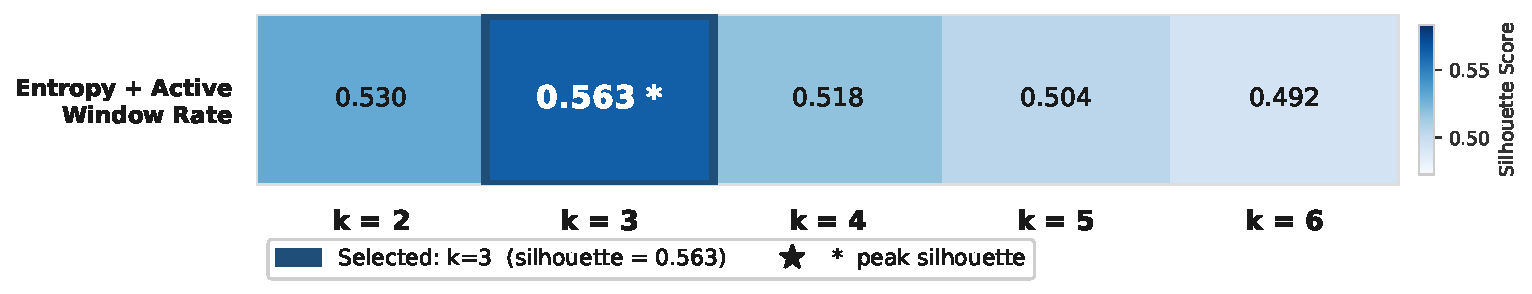
\includegraphics[width=\columnwidth]{silhouette_heatmap_combined.pdf}
    \caption{Silhouette Selection of K }
    \label{fig:Silhouette_analysis}
\end{figure}

\textbf{Consistent Documenters} ($n = 37$, 37\%) maintain
high documentation rhythm across both dimensions with evenly
distributed activity (mean $H_{\text{norm}} = 0.906$) and
persistent presence across the observation window (mean
$AWR = 0.825$).
Documentation was present in approximately
83\% of observed months on average.
\textbf{Occasional Documenters} ($n = 50$, 50\%) represent
the largest and most prevalent archetype, characterized by
moderate entropy (mean $H_{\text{norm}} = 0.762$) and
notably lower active window rate (mean $AWR = 0.440$),
indicating documentation activity concentrated in
approximately 44\% of observed months. Activity occurs in
periodic bursts rather than as a continuous practice, with
extended gaps between documentation efforts. \textbf{Sparse Documenters} ($n = 13$, 13\%) exhibit
near-absent documentation rhythm, with low entropy
(mean $H_{\text{norm}} = 0.546$) and minimal active window
rate (mean $AWR = 0.167$), indicating documentation
activity in approximately one month in six on average.
\vspace{-10pt}
\begin{table}[h]
\centering
\small
\caption{Descriptive statistics for each documentation
rhythm archetype across metrics.}
\label{tab:archetype_stats}
\renewcommand{\arraystretch}{1.3}
\begin{tabular}{lcrrrrr}
\toprule
\textbf{Archetype} & \textbf{n} & \textbf{Metric}
& \textbf{Mean} & \textbf{Median}
& \textbf{Min} & \textbf{Max} \\
\midrule
\multirow{2}{*}{Consistent}
  & \multirow{2}{*}{37}
  & $H_{\text{norm}}$ & 0.906 & 0.908  & 0.832 & 0.989 \\
  &  & $AWR$           & 0.825 & 0.818  & 0.620 & 1.000 \\
\midrule
\multirow{2}{*}{Occasional}
  & \multirow{2}{*}{50}
  & $H_{\text{norm}}$ & 0.762 & 0.758  & 0.647 & 0.848 \\
  &  & $AWR$           & 0.440 & 0.450  & 0.256 & 0.628 \\
\midrule
\multirow{2}{*}{Sparse}
  & \multirow{2}{*}{13}
  & $H_{\text{norm}}$ & 0.546 & 0.534 & 0.406 & 0.637 \\
  &  & $AWR$           & 0.167 & 0.174 & 0.058 & 0.355 \\
\bottomrule
\end{tabular}
\end{table}

The artifacts in Table~\ref{tab:documentation_artifacts} span very different maintenance cadences, from actively-evolving process documentation to write-once legal and attribution files, so we validated the archetype construct against this heterogeneity before treating it as the primary RQ1 result. We partition the 22 artifact types into \textbf{living/process} and \textbf{static/attribution} documentation (full mapping in Table~\ref{tab:artifact_categories}) and recompute entropy and AWR within each stratum. At the ecosystem level, 92.2\% of documentation-touching commits touch only living/process files, and combined-type entropy and AWR correlate with their living-only counterparts at $\rho = 0.93$ and $\rho = 0.94$ (Spearman), respectively, confirming the reported archetypes are driven overwhelmingly by living/process documentation rather than by the inclusion of rarely-touched static files.

\begin{table*}[t]
\centering
\small
\caption{Artifact-to-category mapping used in the living/static robustness check (Rhythm type) and the purpose taxonomy (Purpose). Full artifact descriptions appear in Table~\ref{tab:documentation_artifacts}.}
\label{tab:artifact_categories}
\setlength{\tabcolsep}{6pt}
\renewcommand{\arraystretch}{1.2}
\begin{tabular}{p{2.2cm}p{2.8cm}p{11.5cm}}
\toprule
\textbf{Dimension} & \textbf{Category} & \textbf{Artifacts} \\
\midrule
\multirow{2}{*}{Rhythm type}
 & Living/process & README, CONTRIBUTING, CHANGELOG, HISTORY, RELEASE(S), GOVERNANCE, SECURITY, SUPPORT, MAINTAINERS, CODE\_OF\_CONDUCT, ROADMAP, VISION, BUILDING, COMMIT\_CONVENTIONS, PULL\_REQUEST\_TEMPLATE, ISSUE\_TEMPLATE \\
 & Static/attribution & LICENSE, NOTICE, COPYING, AUTHORS, CREDITS, THANKS, CONTRIBUTORS \\
\midrule
\multirow{4}{*}{Purpose}
 & Onboarding/process & README, CONTRIBUTING, BUILDING, COMMIT\_CONVENTIONS, PULL\_REQUEST\_TEMPLATE, ISSUE\_TEMPLATE \\
 & Governance/policy & GOVERNANCE, CODE\_OF\_CONDUCT, SECURITY, SUPPORT, MAINTAINERS, ROADMAP, VISION \\
 & Change-tracking & CHANGELOG, HISTORY, RELEASE(S) \\
 & Legal/attribution & LICENSE, NOTICE, COPYING, AUTHORS, CREDITS, THANKS, CONTRIBUTORS \\
\bottomrule
\end{tabular}
\end{table*}

% Second, we re-derived rhythm metrics from human-authored commits only, using the author-identity and bot-classification data described in Section~\ref{sec:dataset_const}, since automated processes (e.g., contributor-list bots appending to \texttt{AUTHORS} files) can otherwise be mistaken for sustained governance activity. At the ecosystem level, 7.2\% of documentation-touching commits are bot-authored. We adopt human-authored-only rhythm metrics as the primary analysis throughout this paper (Tables~\ref{tab:descriptive_rhythm_metrics}--\ref{tab:archetype_stats}), which additionally resolves a marginal $k{=}3$/$k{=}4$ tie present in the raw silhouette analysis, leaving $k=3$ as the clear and stable choice. Re-clustering on bot-inclusive data changes the archetype label for only 5 of 100 repositories; the clearest case, \texttt{java-design-patterns}, has 91\% of its documentation commits attributable to a single automated process and shifts from \textit{Consistent} to \textit{Occasional} once excluded, confirming that filtering automated activity, not discarding the archetype construct, is the correct treatment.

\textbf{Documentation Purpose Taxonomy:}
To characterize what "documentation maintenance" concretely consists of, we further partition the 22 artifact types into four purpose-built categories, \textit{onboarding/process}, \textit{governance/policy}, \textit{change-tracking}, and \textit{legal/attribution} (mapping in Table~\ref{tab:artifact_categories}). Change-tracking accounts for the largest ecosystem-level share of commits, but this is driven by a small number of repositories with heavy, often automated, changelog activity: the median repository has \textit{zero} change-tracking commits across the full decade-long window. Onboarding/process documentation, by contrast, is the typical governance activity: it is present in every repository in the sample and accounts for a median 84.6\% of a repository's documentation commits. Governance/policy and legal/attribution activity are minor and frequently absent altogether. This confirms that the ecosystem-level statistics reported throughout this paper (e.g., the 77.9\% DocOnly rate) are numerically anchored in onboarding/process documentation specifically. Table~\ref{tab:artifact_taxonomy} shows that the ecosystem-level and per-repository pictures diverge sharply, and the divergence is itself informative.
\vspace{-10pt}
\begin{table}[h]
\centering
\small
\caption{Documentation purpose taxonomy: ecosystem-level share, median per-repository share, and repositories with zero activity, by category.}
\label{tab:artifact_taxonomy}
\setlength{\tabcolsep}{4pt}
\renewcommand{\arraystretch}{1.2}
\begin{tabular}{lrrr}
\toprule
\textbf{Category} & \textbf{Ecosystem} & \textbf{Median} & \textbf{Zero activity} \\
\midrule
Change-tracking     & 50.8\% & 0.0\%  & 54/100 \\
Onboarding/process  & 41.3\% & 84.6\% & 0/100 \\
Legal/attribution   & 7.7\%  & 3.9\%  & 11/100 \\
Governance/policy   & 3.4\%  & 3.3\%  & 25/100 \\
\bottomrule
\end{tabular}
\end{table}


\begin{tcolorbox}[
  colback=heatmaplight,
  colframe=heatmapdark,
  coltitle=white,
  fonttitle=\bfseries,
  title=Summary — RQ1
]
% The K-Means clustering ($k=3$, silhouette $= 0.603$) on 
% normalized Shannon entropy and active window rate 
% identified \MGuizani{ I suggest starting here in the takeaway to make the findings the main focus especially that the majority lies in the occasional documenter cluster. Really interesting results! we still have a long way to go in documentation... }

Three documentation rhythm archetypes emerged across
100 OSS repositories: \textit{Consistent Documenters}
(37\%), \textit{Occasional Documenters} (50\%), and
\textit{Sparse Documenters} (13\%). The majority of
repositories exhibit occasional rather than consistent
documentation rhythm, with documentation activity present in only 44\% of observed months on average for the largest archetype. We test the durability of these archetypes over time in Section~\ref{sec:evolution}.

\end{tcolorbox}

\subsection{Documentation Intention (RQ2)}

\textbf{Documentation Intention:}
\label{sec:Documentation_Intention}
Across the 100 repositories, health documentation commits constitute a median of only 1.90\% of total commit activity
(mean $= 5.78\%$).
Consequently, we examine how intentionally this documentation activity occurs.

\textbf{Doc-Only Commits:}
Across the 37,447 documentation-touching commits in the decade-long dataset, 29,171 (77.9\%) were documentation only, making this the dominant commit category at the ecosystem level.
At the per-repository level, the documentation-only rate exhibited a left-skewed distribution \textbf{(mean $= 0.785$, median $= 0.825$, SD $= 0.172$)}, indicating that most repositories are concentrated toward the higher end  of the scale.

\textbf{Doc-Dominant and Doc-Non-Dominant Commits:}
Documentation dominant mixed commits modify both health documentation files and other files, but with documentation files constituting at least half of all modified files ($\tau = 0.5$). At the ecosystem level, 4,564 commits (12.2\% of $T$) were classified as documentation-dominant. Documentation non-dominant commits, which modify health documentation files as a minor component of a broader change, accounted for the remaining 3,712 commits (9.9\% of $T$), the smallest of the three categories.
Taken together, documentation-only commits dominate at 77.9\% of all 37,447 documentation touching commits over the decade, followed by documentation-dominant
mixed commits at 12.2\% and non-dominant incidental commits at 9.9\%. Considered alongside the baseline finding that health documentation constitutes a median of \textbf{only 1.90\% of total commit activity}, these proportions establish the central finding that health documentation commits are rare in the context of overall development effort, but when they occur, they are deliberate.
This deliberateness is not static, however; we find it has eroded significantly over the decade studied (Section~\ref{sec:evolution}).

\begin{tcolorbox}[colback=heatmaplight,
                  colframe=heatmapdark,
                  coltitle=white,
                  fonttitle=\bfseries,
                  title=Summary --- RQ2]
When documentation is touched, 90.1\% of those commits are documentation-only or documentation-dominant. Deliberate documentation behavior consistently outweighs incidental contributions, though the documentation-only share has significantly declined over the decade studied.
The core governance challenge is not a lack of intent; contributors document purposefully when they engage. It is rather a lack of frequency, and, increasingly, a lack of intentional documentation practice as projects mature.

\end{tcolorbox}


\subsection{Documentation Ownership (RQ3)}

\textbf{Documentation is a Structural Minority Practice:}
Across the 100 repositories, only 7,988 of 179,622 total contributors (4.5\% at the ecosystem level) ever touched a health documentation file within the decade-long observation window. At the per-repository level, the median participation rate
is \textbf{6.3\%} (mean $= 9.9\%$, SD $= 0.119$,
IQR $= 2.9\%$--$10.9\%$), which implies that the typical project relies on a small minority of its contributors for health documentation governance. Forty-four repositories recorded participation rates below 5\%, and only four exceeded 50\%.
The raw counts reflect this disparity directly: repositories averaged 1,796 total contributors (median $= 1,025$) but only 79.9 documentation contributors (median $= 46$). This participation rate has itself declined significantly over the decade studied (Section~\ref{sec:evolution}).

\textbf{Documentation Ownership is More Concentrated Than Code Ownership:}
Documentation commits are more concentrated than general commit activity across every top-$k$ threshold examined.
The mean top-3 share for documentation commits is
\textbf{0.517} compared to \textbf{0.415} for all commits, with 79 of 100 repositories showing higher documentation concentration. The gap persists at higher $k$: top-5 (0.600 vs.\ 0.484) across 80 repositories and top-10 (0.705 vs.\ 0.577) across 82 repositories. For top-1 share, the single largest documentation contributor accounts for a median of \textbf{25.2\%} of all documentation commits in their repository (mean $= 32.2\%$).
reflecting a subset of projects with extreme
single-contributor dependence even across a full decade of activity.

\textbf{Documentation Governance is Structurally Fragile:}
The documentation bus factor (Bus-50) has a median of \textbf{4} across the 100 repositories (mean $= 8.54$, SD $= 19.53$, IQR $= 2$--$7$). Forty-seven repositories (47\%) have a Bus-50 of three or fewer, this implies that the departure of at most three contributors would shift majority
documentation control. More critically, \textbf{15
repositories (15\%) depend on a single contributor} for the majority of their documentation activity (Bus-50 $= 1$) even across a full decade.
Bus-80 confirms the broader fragility, the median repository requires only 16 contributors to account for 80\% of documentation commits,
and 35 of repositories (35\%)  reach that threshold with 10 or fewer. Bus-50 correlates strongly with total contributor count ($\rho = +0.58$, $p < 0.0001$), confirming that larger repositories naturally attract more documentation contributors and distribute ownership more broadly, and neither entropy nor active window rate add explanatory power over contributor count alone, consistent with our RQ1 finding that documentation rhythm and ownership concentration are largely independent dimensions of governance.

% \EAdejumo{New subsection: file-centric bus factor robustness check, giving the fragility claim a second, methodologically distinct estimate.}
% \subsubsection{\textbf{File-Centric Ownership Validation}}
% The bus factor above is computed from aggregate commit counts across all health documentation files touched by a contributor, following Cosentino et al.~\cite{cosentino2015assessing}. As a methodologically distinct robustness check, closer to Jabrayilzade et al.'s~\cite{jabrayilzade2022bus} file-level treatment of ownership, we additionally compute a \textbf{file-centric} bus factor: for each health-documentation file we identify its top-commit-count owner, then compute Bus-50/80 as the minimum number of distinct primary file owners needed to collectively be the top owner of at least 50\%/80\% of a repository's touched health documentation files. This shifts the unit of ownership from aggregate activity to per-file primary responsibility.

% The file-centric measure correlates moderately with the commit-count measure (Spearman $\rho = 0.468$, $p < 0.0001$ for Bus-50; $\rho = 0.548$, $p < 0.0001$ for Bus-80), close enough to indicate both capture the same underlying construct, yet distinct enough to serve as a genuine robustness check rather than a restatement. Critically, the file-centric method reveals \textit{more}, not less, structural fragility: 55.1\% of repositories (54 of the 98 with file-level ownership data available) have a file-centric Bus-50 of 1, compared to 27.6\% under the commit-count method on the same 98 repositories. Read together, the two measures indicate that our headline estimate, 28\% of repositories dependent on a single contributor, is if anything conservative: examining who primarily owns each individual health-documentation file surfaces single-point-of-failure risk in over half of the repositories studied.

\textbf{Ownership Structure Predicts Documentation Outcomes}
\label{sec:predictive_validity}
Using the outcome-validation methodology (Section~\ref{sec:outcome_validation}), we tested whether documentation participation rate, documentation bus factor, entropy, and active window rate predict documentation staleness, contributor retention, and repository-wide project health outcomes (general contributor retention, newcomer arrival, contributor growth, maintainer turnover, and overall activity trend) across the full decade of observation. Documentation rhythm archetype shows strong bivariate associations with several of these outcomes, but every one is fully explained by contributor ecosystem size and adds no explanatory power in a confound-controlled test. Three relationships, however, survive the full four-check battery (Table~\ref{tab:predictive_validity}).

\vspace{-6pt}
\begin{table}[h]
\centering
\small
\caption{Confound-control battery ($p$-values) for the three validated predictor--outcome relationships. A relationship is reported as validated only if it survives all four checks (Section~\ref{sec:outcome_validation}).}
\label{tab:predictive_validity}
\setlength{\tabcolsep}{3pt}
\renewcommand{\arraystretch}{1.25}
\begin{tabular}{p{3.1cm}cccc}
\toprule
\textbf{Predictor $\rightarrow$ Outcome} & \textbf{Size} & \textbf{Volume} & \textbf{Robust} & \textbf{Outlier} \\
\midrule
Bus factor $\rightarrow$ Staleness & 0.0015 & 0.0015 & 0.0038 & 0.0031 \\
Participation $\rightarrow$ Retention & $<$0.001 & $<$0.001 & $<$0.001 & $<$0.001 \\
Participation $\rightarrow$ Activity trend & 0.027 & 0.009 & 0.019 & 0.012 \\
\bottomrule
\end{tabular}
\end{table}
\vspace{-6pt}

\textbf{Bus factor predicts documentation freshness.} Documentation bus factor predicts staleness across all four checks in Table~\ref{tab:predictive_validity}: repositories with a \textit{higher} bus factor, documentation responsibility spread across more contributors rather than concentrated in one or two, keep their documentation measurably fresher (partial $\rho = -0.394$, a moderate negative association; significance comes from the four checks, not from the size of $\rho$ alone). Entropy and active window rate show a similar bivariate pattern but do not clear the battery once documentation volume is controlled, and participation rate alone does not survive robust standard errors ($p = 0.090$). Ownership concentration, not the raw volume or rhythm of documentation activity, is what most reliably distinguishes repositories that keep documentation current from those that do not.

\textbf{Participation breadth predicts \textit{lower} newcomer retention.} A construct-matched test, predicting whether documentation newcomers return to touch documentation again rather than a domain-mismatched general-activity outcome, shows documentation participation rate predicts newcomer retention across all four checks (Table~\ref{tab:predictive_validity}), and the same battery rerun on the stricter subsample of repositories with at least 10 documentation newcomers ($n=89$) reproduces it. The direction, however, is negative: repositories where a \textit{larger} share of the contributor base ever touches documentation retain a \textit{smaller} proportion of their individual documentation newcomers ($\beta = -0.618$, partial $\rho = -0.200$). The association is directionally stable across every specification we examined, including with no controls at all ($\beta = -0.217$, $p = 0.045$), so it is not an artifact of the confound-control design. In practical terms, moving across the interquartile range of participation rate (2.9\% to 10.5\%) corresponds to a 4.7 percentage-point fall in newcomer retention, against a sample mean retention rate of 25.5\%.

We read this as a composition effect rather than evidence that broad participation drives newcomers away. A repository where documentation is touched by a wide slice of the contributor base is, by construction, one where many contributors make a single incidental documentation edit, a typo correction or a one-line README fix, without that edit marking the start of sustained documentation involvement. Breadth and per-newcomer persistence are therefore in tension: the same openness that admits many casual documentation contributors also dilutes the share of them who return. Bus factor's relationship with retention does not clear the same battery in either the contemporaneous or a temporally-lagged design (bus factor computed on only the first half of the observation window, predicting established-contributor loss in the second half), so concentration offers no corresponding lever on retention in either direction.

\textbf{Participation breadth is weakly associated with overall project activity.} Documentation participation rate also predicts the repository's general activity trend, the slope of overall monthly commit volume across the decade, and no other governance predictor, including documentation bus factor and rhythm archetype, survives the same battery against a general project-health outcome. We report this association with two explicit caveats. First, it is detectable only net of project size: the raw, uncontrolled association is negative and non-significant ($\beta = -0.009$, $p = 0.31$) and turns positive once contributor count enters the model ($\beta = +0.022$, $p = 0.027$). This reversal is interpretable, participation rate is itself strongly negatively correlated with project size ($r = -0.593$) while size is positively correlated with activity trend ($r = +0.443$), so size suppresses the relationship in the raw data, but it does mean the finding is a statement about repositories \textit{of comparable size} rather than a pattern visible in the ecosystem at large. Second, the effect is small: the partial rank correlation is near zero ($\rho = +0.014$), and moving across the interquartile range of participation rate shifts the activity trend by roughly 0.21 standard deviations of that outcome. We therefore treat this as suggestive evidence that documentation participation carries information about project trajectory beyond documentation itself, not as a robust predictive claim on the order of the two findings above.

\textbf{Scope of the validated claims:} Ownership structure carries genuine predictive value, but its two facets do not simply point the same way. Concentration (bus factor) predicts documentation currency: spreading documentation responsibility keeps documentation fresher. Breadth (participation rate) is double-edged: the wider the slice of contributors that touches documentation, the smaller the proportion of individual documentation newcomers who return, even as breadth is weakly associated with a healthier overall project trajectory. Documentation governance therefore admits no single dominant lever, and in particular no evidence here supports treating broad participation as uniformly beneficial. The raw volume and temporal rhythm of documentation activity, by contrast, do not independently predict any of these outcomes once size and volume are controlled.


\begin{tcolorbox}[
  colback=heatmaplight,
  colframe=heatmapdark,
  coltitle=white,
  fonttitle=\bfseries,
  title=Summary --- RQ3
]
Health documentation is maintained by a
minority of contributors, and that minority has been shrinking. The median repository
has only 6.3\% of its contributor pool engaging with health documentation (ecosystem rate $= 4.5\%$), a rate that has declined significantly over the decade studied. Among those who
do document, ownership is more concentrated than general code ownership at every top-$k$ level. 15\% of repositories depend on a single contributor for the majority of documentation commits (Bus-50 $= 1$) even across a full decade. Ownership structure carries genuine predictive value, but its two facets pull in different directions: a higher documentation bus factor independently predicts fresher documentation, while broader participation predicts \textit{lower} retention of individual documentation newcomers, and is only weakly associated with a healthier overall activity trend. Breadth buys reach at the cost of per-newcomer persistence.
\end{tcolorbox}

\subsection{Documentation Governance Evolution (RQ4)}
\label{sec:evolution}
RQ1--RQ3 characterize documentation governance as it stands across the decade studied. Using the annual classification and trend-testing procedures described in Section~\ref{sec:RQ4}, we test whether each dimension, rhythm, intention, and ownership, is stable or shifting over time.

\textbf{Rhythm is durable.} Table~\ref{tab:transition_matrix} reports the pooled adjacent-year transition matrix across all 710 valid consecutive year-pairs. Consistent Documenters remain Consistent the following year 76.3\% of the time and Sparse Documenters remain Sparse 61.7\% of the time; Occasional Documenters persist only 37.6\% of the time, more often drifting toward Sparse (43.1\%) than remaining Occasional. Comparing each repository's earliest to latest valid year ($n=98$ repositories with at least two valid years) shows the same ordering at a coarser grain: 46.8\% decade-long persistence for Consistent, 73.3\% for Sparse, and only 33.3\% for Occasional. Consistent and Sparse behave as self-reinforcing, sticky states, while Occasional is a transitional state repositories pass through rather than settle into, and one that drains toward Sparse far more often than it climbs toward Consistent.

\vspace{-6pt}
\begin{table}[h]
\centering
\small
\caption{Adjacent-year rhythm archetype transition matrix (row-normalized \%, pooled across 710 valid consecutive year-pairs). Rows are the archetype in year $y$, columns the archetype in year $y{+}1$.}
\label{tab:transition_matrix}
\setlength{\tabcolsep}{4pt}
\renewcommand{\arraystretch}{1.2}
\begin{tabular}{lrrrr}
\toprule
\textbf{From $\downarrow$\, To $\rightarrow$} & \textbf{Consistent} & \textbf{Occasional} & \textbf{Sparse} & \textbf{n} \\
\midrule
Consistent & 76.3\% & 18.7\% & 5.0\%  & 299 \\
Occasional & 19.3\% & 37.6\% & 43.1\% & 202 \\
Sparse     & 6.7\%  & 31.6\% & 61.7\% & 209 \\
\bottomrule
\end{tabular}
\end{table}
\vspace{-6pt}

\textbf{Intentionality is eroding.} The documentation-only rate declines significantly year over year. The per-repository-year association is weak (Spearman $\rho = -0.076$, $p = 0.027$); the trend is clearest in central tendency, where the Mann-Kendall test on the annual median is significant (Mann-Kendall $p = 0.003$) and the annual median itself falls from 87.7\% in the first year of the window to 75.0\% in the final year, a 12.7-point decline.

\textbf{Ownership breadth is narrowing.} Documentation participation rate shows the same declining pattern. As above, the per-observation association is small (Spearman $\rho = -0.126$, $p = 0.0001$), while the Mann-Kendall test on the annual median is the more direct evidence of the trend ($p = 0.0007$): the annual median falls from 7.1\% to 4.3\% across the same window, a 2.8-point decline that amounts to a 39\% relative drop off the starting rate.

Rhythm archetypes entrench once established, while the breadth and deliberateness of documentation engagement both erode as projects mature; these are divergent trajectories along the same decade, the coarse label a project carries becomes more entrenched even as the people and deliberateness sustaining it thin out. Section~\ref{sec:Discussion} discusses the implications of this combination alongside our predictive-validity results.

\begin{tcolorbox}[
  colback=heatmaplight,
  colframe=heatmapdark,
  coltitle=white,
  fonttitle=\bfseries,
  title=Summary --- RQ4
]
Documentation governance is not static. Rhythm archetypes are self-reinforcing: once a repository becomes a Consistent or Sparse Documenter, it is more likely than not to remain one the following year (76\% and 62\% respectively), while Occasional functions as a transitional state that drains toward Sparse more often than it climbs toward Consistent. At the same time, both the deliberateness (DocOnly rate, $-$12.7 points) and breadth (participation rate, $-$2.8 points) of documentation engagement have eroded significantly over the same decade. Documentation governance is entrenching in its coarse rhythm while narrowing in who sustains it and how deliberately.
\end{tcolorbox}

\section{Discussion}
\label{sec:Discussion}

Existing OSS health tooling such as CHAOSS~\cite{chaoss} tracks dozens of code-centric metrics, commit frequency, issue responsiveness, pull request throughput, but has no equivalent for documentation, despite documentation bus factor, participation rate, and rhythm archetype each being computable from data these frameworks already ingest. The three findings below make concrete why that gap matters.

\noindent \textbf{Ownership Structure and Its Downstream Consequences:} Documentation rhythm captures the currency
of health artifacts over time; a project transitioning toward Sparse rhythm has governance documentation that increasingly fails to reflect current project norms, raising the onboarding barriers that prior work has linked to newcomer dropout and
contributor attrition~\cite{steinmacher2015social,steinmacher2014attracting}. Our outcome-validation results (Section~\ref{sec:predictive_validity}) substantiate this connection directly for ownership concentration rather than leaving it implicit: repositories with a higher documentation bus factor, ownership spread across more contributors rather than concentrated in one or two, keep their documentation measurably fresher, controlling for both community size and how much documentation work is produced overall, and our finding that 15\% of repositories have Bus-50$=1$ for documentation, even measured across a full decade, indicates that governance fragility is widespread even among the most mature projects studied. Participation breadth, in turn, predicts a different outcome in the opposite direction: repositories where a wider slice of contributors touches documentation retain a \textit{smaller} share of their individual documentation newcomers. Read as a composition effect, breadth admits many one-off documentation contributors whose single edit does not begin sustained involvement, so the two facets of ownership structure trade against one another rather than reinforcing: concentration keeps documentation current, while breadth buys reach at the cost of per-newcomer persistence. Practitioners cannot therefore maximize both at once, and a project that deliberately widens documentation participation should expect its per-newcomer return rate to fall even as its documentation reaches more hands.

\noindent \textbf{Entrenchment Meets Erosion: A Narrowing Window for Intervention:} Our RQ4 results compound rather than merely coexist. Rhythm archetypes are self-reinforcing once established: an Occasional repository is more likely to drift toward Sparse (43\% of adjacent-year transitions) than to climb toward Consistent (19\%), whether measured year-to-year or across the full decade span. At the same time, the two levers most associated with staying out of that drift, breadth of contributor participation and deliberateness of documentation effort, are themselves eroding ecosystem-wide. Because documentation participation rate is also the one governance signal in this study that independently predicts a repository's overall activity trend, not just documentation-specific outcomes, its decline is plausibly not only a documentation symptom but an early signal of broader project trajectory, a leading indicator fading precisely where our health-framework recommendation above would make it visible. Practically, this argues for treating a Consistent-to-Occasional rhythm shift, or a falling participation rate, as an actionable trigger for succession planning around single-owner documentation and for deliberate onboarding investment in documentation specifically, rather than as a lagging description of decline already underway.

\noindent \textbf{Automated Documentation Synchronization:} Closing the metrics gap noted above is necessary but not sufficient: metrics that make documentation risk visible only help if something acts on them before the window closes. Documentation participation breadth, not volume or rhythm, is the governance dimension our results tie most directly to who engages with documentation at all, and it is this same breadth that is eroding ecosystem-wide. That creates a specific risk for how automation gets designed: tooling that keeps documentation technically current without broadening who touches it, an automated changelog or LLM-drafted README update~\cite{adejumo2026bridging,adejumo2024towards}, for instance, would optimize our bus-factor-currency finding while leaving participation breadth untouched or narrowing it further. The more defensible target is not full substitution of human maintainers but automation that surfaces documentation obligations at the point of code change to contributors who have not yet engaged with documentation, rather than routing them to the same one or two maintainers who already carry disproportionate ownership. Built this way, automated synchronization could counteract the concentration our RQ3 results identify as fragile, rather than reinforcing it.


\section{Threats to Validity}
\label{sec:Threats_to_Validity}

\subsection{Internal Threats}
\textbf{External Documentation:}
Our analysis was confined to repository resident observable health documentation related files. Manual inspection of the 100 repositories identified 20 projects that specifically host contributing related artifacts, a crucial health documentation on external websites or wikis rather than as in-repository files. This limitation is inherent in repository mining studies and in our study affects rhythm, intention, and ownership metrics uniformly across impacted repositories.

% \subsubsection{Association, Not Causation, in the Retention Finding}
% The bus-factor--retention relationship in Section~\ref{sec:predictive_validity} is reported as an association, and the temporally-ordered (lagged) design rules out one specific alternative explanation, the outcome mechanically determining the predictor, but it cannot rule out an unobserved shared cause (for example, smaller, more intimate contributor communities independently producing both concentrated ownership and higher retention) driving both quantities together. We report the finding as robust and directionally consistent across two populations and two temporal designs, not as a demonstrated causal mechanism.

\subsection{External Threats}
\textbf{Repository Selection and Generalization}
Our selection criteria requiring more than 10,000 stars, 9,000 forks, and ten years of history deliberately sample mature, high-visibility projects that benefit from large contributor communities and established governance cultures. Findings should not be generalized directly to smaller or younger repositories, where documentation fragility is likely more acute. We treat this as a conservative bound, if governance is structurally fragile even in the most successful OSS projects, the problem is likely
worse across the ecosystem at large. 




\section{Conclusion and Future Work}
\label{sec:conclusion}
% \EAdejumo{Conclusion rewritten: predictive validation is now reported as an accomplished result rather than deferred future work, and the future-work list is revised accordingly.}
This paper establishes documentation governance as a measurable, multi-dimensional, and evolving construct in OSS that is rare, deliberate, and structurally fragile, and shows that documentation bus factor independently predicts documentation staleness while documentation participation breadth independently predicts \textit{lower} retention of individual documentation newcomers, both beyond project size and activity volume, a reach-versus-persistence tradeoff rather than a single dominant governance lever. Our decade-long observation window further reveals that documentation governance is not static: rhythm archetypes are durable and self-reinforcing rather than incidental, even as documentation participation and deliberateness have each declined significantly over the ten years studied \textbf{(RQ4)}. Several questions remain open. The relationships we identify are associational, not causal; establishing their causal structure, and specifically whether documentation ownership structure can be deliberately cultivated to improve both currency and retention simultaneously, is a natural next step, potentially through matched-repository or interventional designs. Extending the analysis to smaller and younger repositories will improve generalization.

% Whether consistent documentation rhythm is achievable without
% organizational backing, and whether automated tooling, staleness alerts, documentation bus factor dashboards, succession-planning support for single-owner documentation, or LLM-assisted governance gap detection, can compensate for the structural fragility we observe while preserving the retention benefits associated with it, remain open and practically consequential questions.
\subsection{Data Availability Statement: }
Our replication package is made available: \cite{replication}. 

% EAdejumo: bibliography style switched to IEEEtran (references.bib and \cite keys are unchanged
% and do not need editing; only the style file governing reference formatting changes).
\bibliographystyle{IEEEtran}
\bibliography{references}


\end{document}
